\chapter{Testing and Evaluation}
\label{chapter5}

\section{Test Cases}

In order to test the load balancing application, test scenarios were designed to see how it would effect real world cases. Using the virtual network created with the mininet program and the iperf network bandwidth measurement tool, traffic is generated between the player hosts and game server hosts. The bandwidth of this traffic will be based on network requirements suggestions for 1080p at 60FPS, 720p at 60FPS and 720p at 30FPS given by nVidia's GeForce Now cloud gaming system requirements \cite{nvidiasysreq} as shown in Table \ref{table:traffic}. The iperf tool used to generate the traffic will set the player hosts in server mode and the game servers in client mode. This is so the game server can send UDP traffic to it's connected player host machine. UDP is used since its traffic bandwidth can be set and is the protocol that is used for streaming video data over TCP. 
\newline
\par
Latency will be simply tested by sending 10 ping requests from player host to game server whilst the iperf traffic is being sent. Each test case will contain multiple tests using each of the settings in Table \ref{table:traffic} with tests before load balancing and then with load balancing in effect. To make sure th tests without load balancing doesn't depend on routes specified by previous load balanced runs, flows created by previous load balanced runs are deleted using a python script that makes REST API calls to the OpenDaylight SDN controller.

\begin{table}[h!]
\centering
\begin{tabular}{|l|l|}
\hline
\textbf{\begin{tabular}[c]{@{}l@{}}Video\\ Settings\end{tabular}} & \textbf{\begin{tabular}[c]{@{}l@{}}Network\\ Bandwidth\end{tabular}} \\ \hline
1080p + 60FPS                                                     & 50 Mbps                                                              \\ \hline
720p + 60FPS                                                      & 30 Mbps                                                              \\ \hline
720p + 30FPS                                                      & 10 Mbps                                                              \\ \hline
\end{tabular}
\caption{Traffic Simulation Settings}
\label{table:traffic}
\end{table}

\subsection{Case 1}
The first case is two players using the cloud gaming system with their game instance being in two separate servers but under the same switch. Player host 1 'h1' (10.0.0.1) and player host 2 'h2' (10.0.0.2) are used and are connected to 'h4' (10.0.0.4) and 'h5' (10.0.0.5) respectively. This shows a basic example of multiple players connected to different game servers but using the same Top of the Rack switch. As shown in Figure \ref{fig:test1}, there are two possible routes for traffic flowing from the core switch 's1' to switch 's4' (1::2::4 and 1::3::4). When the load balancer is running for each flow, it will assign a different route for each of them. Figure \ref{fig:test1} shows one out of the two possible load balanced routes with the other being just a swap with the red and blue path between 's1' and 's4' switches.

\begin{figure}[h!]
 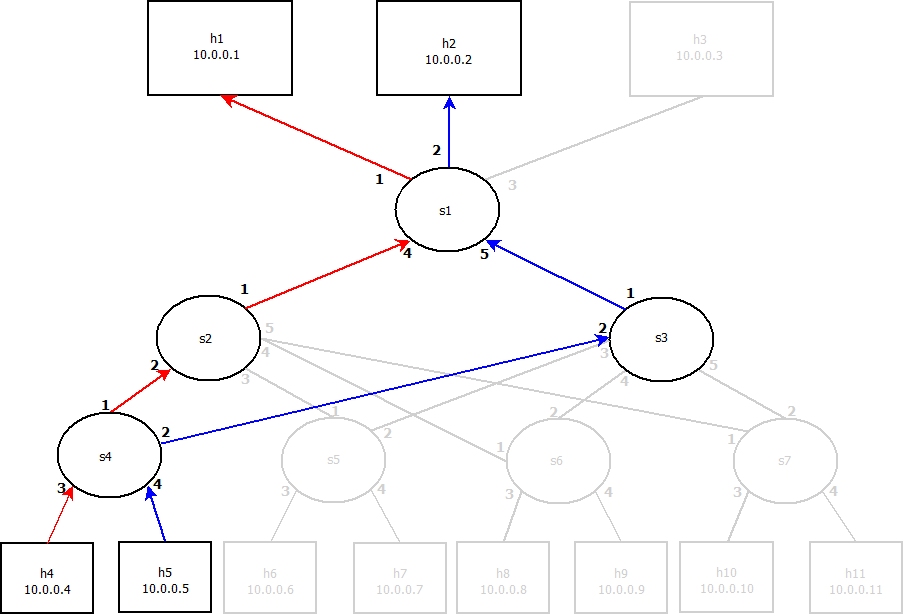
\includegraphics[width=\linewidth]{images/test1.png}
 \caption{Test Case 1: Possible load balanced routes}
 \label{fig:test1}
\end{figure}

\subsection{Case 2}
The second case is when two players are connected to the same physical game server host since it can contain multiple virtual machines with multiple game instances. Also it can represent two players playing the same game instance such as a multiplayer game so two video traffic will be needed to be generated and sent to the two separate clients. For this test case, hosts 'h1' and 'h2' will be used to be connected to host 'h4'. The possible load balanced routes between the switches will be the same as in test case 1 but with two separate traffic being generated from 'h4' as shown in Figure \ref{fig:test2}.

\begin{figure}[h!]
 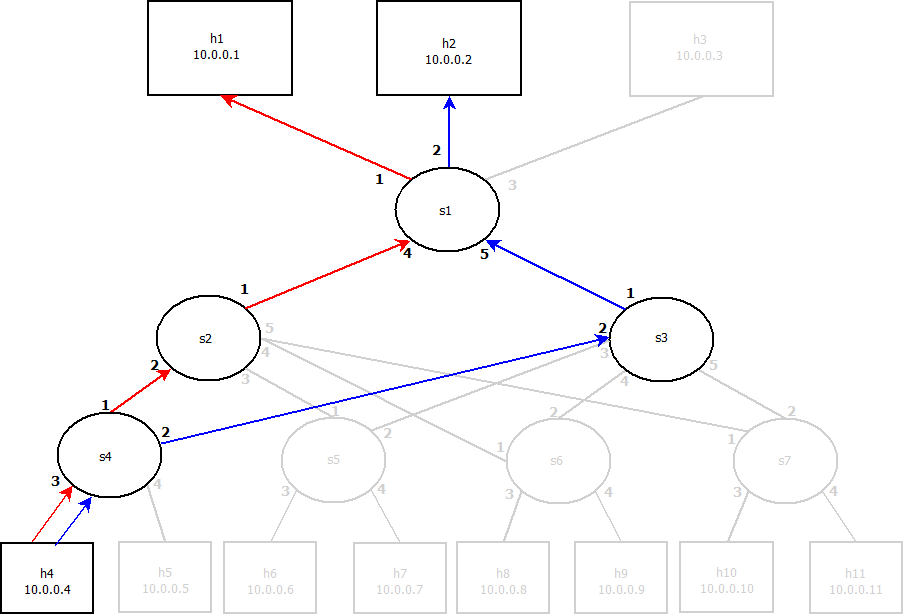
\includegraphics[width=\linewidth]{images/test2.png}
 \caption{Test Case 2: Possible load balanced routes}
 \label{fig:test2}
\end{figure}

\subsection{Case 3}
\lipsum[1-1]





\begin{figure}[h]
 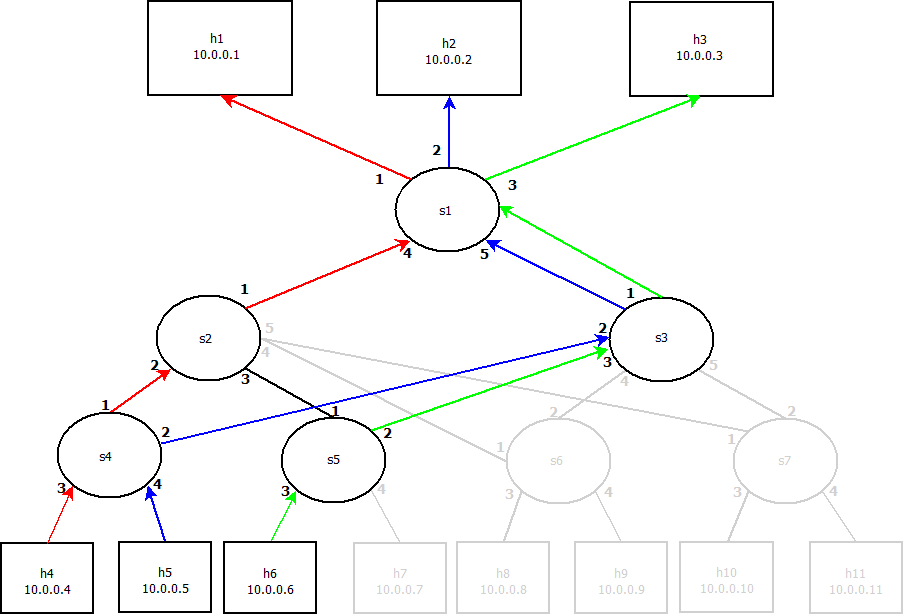
\includegraphics[width=\linewidth]{images/test3.png}
 \caption{Test Case 3: Possible load balanced routes}
 \label{fig:test3}
\end{figure}

\section{Results}

\begin{table}[h!]
\centering
\begin{tabular}{l|l|l|l|l|l|l|l|l|}
\cline{2-9}
                                                   & \multicolumn{4}{c|}{\textbf{Before Load Balancing}}                                                                                            & \multicolumn{4}{c|}{\textbf{With Load Balancing}}                                                                                              \\ \hline
\multicolumn{1}{|c|}{\textbf{Connection}}          & \multicolumn{1}{c|}{\textbf{min}} & \multicolumn{1}{c|}{\textbf{avg}} & \multicolumn{1}{c|}{\textbf{max}} & \multicolumn{1}{c|}{\textbf{mdev}} & \multicolumn{1}{c|}{\textbf{min}} & \multicolumn{1}{c|}{\textbf{avg}} & \multicolumn{1}{c|}{\textbf{max}} & \multicolumn{1}{c|}{\textbf{mdev}} \\ \hline
\multicolumn{9}{|c|}{\textbf{50 Mbps}}                                                                                                                                                                                                                                                                                                               \\ \hline
\multicolumn{1}{|l|}{\textbf{h1 -\textgreater h4}} & 210.317                           & 223.223                           & 244.866                           & 9.440                              & 37.409                            & 40.268                            & 47.533                            & 2.685                              \\ \hline
\multicolumn{1}{|l|}{\textbf{h2 -\textgreater h5}} & 278.072                           & 280.276                           & 281.873                           & 1.522                              & 265.200                           & 269.559                           & 274.839                           & 2.182                              \\ \hline
\multicolumn{9}{|c|}{\textbf{30 Mbps}}                                                                                                                                                                                                                                                                                                               \\ \hline
\multicolumn{1}{|l|}{\textbf{h1 -\textgreater h4}} & 57.012                            & 75.600                            & 108.208                           & 15.111                             & 36.755                            & 37.891                            & 41.927                            & 1.428                              \\ \hline
\multicolumn{1}{|l|}{\textbf{h2 -\textgreater h5}} & 274.877                           & 280.685                           & 286.498                           & 4.096                              & 36.628                            & 38.28                             & 45.249                            & 2.373                              \\ \hline
\multicolumn{9}{|c|}{\textbf{10 Mbps}}                                                                                                                                                                                                                                                                                                               \\ \hline
\multicolumn{1}{|l|}{\textbf{h1 -\textgreater h4}} & 41.814                            & 43.108                            & 46.786                            & 1.469                              & 37.211                            & 38.107                            & 39.057                            & 0.596                              \\ \hline
\multicolumn{1}{|l|}{\textbf{h2 -\textgreater h5}} & 42.486                            & 43.516                            & 44.502                            & 0.675                              & 37.550                            & 38.200                            & 39.239                            & 0.653                              \\ \hline
\end{tabular}
\caption{Test Case 1 Results}
\label{table:test1}
\end{table}

\begin{table}[h!]
\centering
\begin{tabular}{l|l|l|l|l|l|l|l|l|}
\cline{2-9}
                                                   & \multicolumn{4}{c|}{\textbf{Before Load Balancing}}                                                                                            & \multicolumn{4}{c|}{\textbf{With Load Balancing}}                                                                                              \\ \hline
\multicolumn{1}{|c|}{\textbf{Connection}}          & \multicolumn{1}{c|}{\textbf{min}} & \multicolumn{1}{c|}{\textbf{avg}} & \multicolumn{1}{c|}{\textbf{max}} & \multicolumn{1}{c|}{\textbf{mdev}} & \multicolumn{1}{c|}{\textbf{min}} & \multicolumn{1}{c|}{\textbf{avg}} & \multicolumn{1}{c|}{\textbf{max}} & \multicolumn{1}{c|}{\textbf{mdev}} \\ \hline
\multicolumn{9}{|c|}{\textbf{50 Mbps}}                                                                                                                                                                                                                                                                                                               \\ \hline
\multicolumn{1}{|l|}{\textbf{h1 -\textgreater h4}} & 268.850                           & 296.824                           & 320.158                           & 18.250                             & 209.526                           & 213.216                           & 216.632                           & 3.011                              \\ \hline
\multicolumn{1}{|l|}{\textbf{h2 -\textgreater h4}} & 357.026                           & 377.026                           & 404.797                           & 20.273                             & 272.451                           & 274.735                           & 275.937                           & 1.167                              \\ \hline
\multicolumn{9}{|c|}{\textbf{30 Mbps}}                                                                                                                                                                                                                                                                                                               \\ \hline
\multicolumn{1}{|l|}{\textbf{h1 -\textgreater h4}} & 213.000                           & 221.689                           & 229.219                           & 6.238                              & 38.468                            & 39.232                            & 39.960                            & 0.448                              \\ \hline
\multicolumn{1}{|l|}{\textbf{h2 -\textgreater h4}} & 296.504                           & 302.919                           & 321.211                           & 7.733                              & 38.525                            & 39.243                            & 39.995                            & 0.469                              \\ \hline
\multicolumn{9}{|c|}{\textbf{10 Mbps}}                                                                                                                                                                                                                                                                                                               \\ \hline
\multicolumn{1}{|l|}{\textbf{h1 -\textgreater h4}} & 42.832                            & 43.443                            & 44.234                            & 0.484                              & 39.985                            & 38.016                            & 38.572                            & 0.432                              \\ \hline
\multicolumn{1}{|l|}{\textbf{h2 -\textgreater h4}} & 41.622                            & 42.396                            & 44.543                            & 0.936                              & 36.992                            & 38.007                            & 39.062                            & 0.739                              \\ \hline
\end{tabular}
\caption{Test Case 2 Results}
\label{table:test2}
\end{table}

\begin{table}[h!]
\centering
\begin{tabular}{l|l|l|l|l|l|l|l|l|}
\cline{2-9}
                                                   & \multicolumn{4}{c|}{\textbf{Before Load Balancing}}                                                                                            & \multicolumn{4}{c|}{\textbf{With Load Balancing}}                                                                                              \\ \hline
\multicolumn{1}{|c|}{\textbf{Connection}}          & \multicolumn{1}{c|}{\textbf{min}} & \multicolumn{1}{c|}{\textbf{avg}} & \multicolumn{1}{c|}{\textbf{max}} & \multicolumn{1}{c|}{\textbf{mdev}} & \multicolumn{1}{c|}{\textbf{min}} & \multicolumn{1}{c|}{\textbf{avg}} & \multicolumn{1}{c|}{\textbf{max}} & \multicolumn{1}{c|}{\textbf{mdev}} \\ \hline
\multicolumn{9}{|c|}{\textbf{50 Mbps}}                                                                                                                                                                                                                                                                                                               \\ \hline
\multicolumn{1}{|l|}{\textbf{h1 -\textgreater h4}} & 208.303                           & 216.48                            & 220.662                           & 4.465                              & 37.631                            & 40.998                            & 49.488                            & 3.256                              \\ \hline
\multicolumn{1}{|l|}{\textbf{h2 -\textgreater h5}} & 269.297                           & 273.377                           & 277.458                           & 4.113                              & 269.133                           & 272.394                           & 274.474                           & 2.096                              \\ \hline
\multicolumn{1}{|l|}{\textbf{h3 -\textgreater h6}} & 426.205                           & 435.244                           & 443.197                           & 6.979                              & 421.068                           & 424.151                           & 425.826                           & 1.589                              \\ \hline
\multicolumn{9}{|c|}{\textbf{30 Mbps}}                                                                                                                                                                                                                                                                                                               \\ \hline
\multicolumn{1}{|l|}{\textbf{h1 -\textgreater h4}} & 205.742                           & 210.754                           & 216.244                           & 3.768                              & 36.542                            & 38.055                            & 40.507                            & 1.168                              \\ \hline
\multicolumn{1}{|l|}{\textbf{h2 -\textgreater h5}} & 271.333                           & 273.377                           & 278.936                           & 2.629                              & 36.397                            & 37.288                            & 38.337                            & 0.657                              \\ \hline
\multicolumn{1}{|l|}{\textbf{h3 -\textgreater h6}} & 425.217                           & 427.494                           & 431.469                           & 2.499                              & 425.185                           & 426.292                           & 430.231                           & 1.489                              \\ \hline
\multicolumn{9}{|c|}{\textbf{10 Mbps}}                                                                                                                                                                                                                                                                                                               \\ \hline
\multicolumn{1}{|l|}{\textbf{h1 -\textgreater h4}} & 41.517                            & 42.602                            & 44.918                            & 0.966                              & 37.082                            & 38.156                            & 40.023                            & 0.975                              \\ \hline
\multicolumn{1}{|l|}{\textbf{h2 -\textgreater h5}} & 41.602                            & 43.132                            & 44.731                            & 0.943                              & 37.598                            & 38.386                            & 38.999                            & 0.387                              \\ \hline
\multicolumn{1}{|l|}{\textbf{h3 -\textgreater h6}} & 426.631                           & 428.373                           & 430.332                           & 1.518                              & 36.981                            & 37.702                            & 38.944                            & 0.523                              \\ \hline
\end{tabular}
\caption{Test Case 3 Results}
\label{table:test3}
\end{table}

\section{Evaluation}
\lipsum[1-1]